\documentclass{beamer}

\usepackage{graphbox}
\usepackage{nth}

\newcommand{\backupbegin}{
   \newcounter{finalframe}
   \setcounter{finalframe}{\value{framenumber}}
}
\newcommand{\backupend}{
   \setcounter{framenumber}{\value{finalframe}}
}
\newcommand\blfootnote[1]{%
  \begingroup
  \renewcommand\thefootnote{}\footnote{#1}%
  \addtocounter{footnote}{-1}%
  \endgroup
}

\usetheme{metropolis}
\setbeamercolor{background canvas}{bg=white}

\title{\includegraphics[align=c,width=.1\textwidth]{../../logo/signal.png}~IHR: Monitoring Internet Health at Scale
\\\hfill \small{\url{https://ihr.iijlab.net}}}

\author[shortname]{\textbf{Romain Fontugne}\\IIJ Research Lab}
%\institute{IIJ Research Lab}

\date{\vfill\hfill\vspace{-1cm}\scriptsize{JFLI – Tokyo Tech Workshop 2019} }
% Used with singapore template
%\titlegraphic{\includegraphics[width=.15\textwidth]{../../logo/signal.png}\\~\\} 
%\beamertemplatenavigationsymbolsempty


\setbeamertemplate{footline}[frame number]
\begin{document}
\frame[plain,noframenumbering]{\titlepage}


\frame{
\frametitle{Internet: a network of networks}
\begin{block}{}
\begin{overlayarea}{\textwidth}{.7\textheight}
    \only<1>{\includegraphics[width=\columnwidth]{../../tartiflette/imc17/fig/tartiflette_background.pdf}}
    \only<2>{\includegraphics[width=\columnwidth]{../../tartiflette/imc17/fig/tartiflette_complaints.pdf}}
    \only<3>{\includegraphics[width=\columnwidth]{../../tartiflette/imc17/fig/tartiflette_operator.pdf}}
\end{overlayarea}
\end{block}
}

\frame{
    \frametitle{Internet Health Report?}

    \begin{block}{Goal: Monitor Internet's Health}
        \begin{itemize}
            \item Automatically pinpoint connectivity issues
        \end{itemize}
    \end{block}

    \begin{columns}
        \column{.6\textwidth}
        \begin{block}{Main Challenges:}
            \begin{itemize}
                \item Internet is huge 
                    \begin{itemize}
                        \item Over 60k autonomous systems
                        \item Billions of connected devices
                    \end{itemize}
                \item Constantly evolving 
                \item Limited views on remote networks
            \end{itemize}
        \end{block}
        \column{.3\textwidth}
        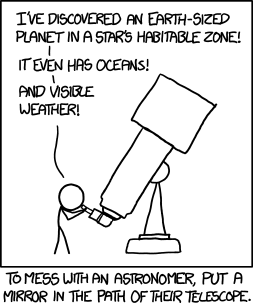
\includegraphics[width=\textwidth]{fig/xkcd_telescope.png}
    \end{columns}
}

\frame{
    \frametitle{Internet Health Report: Current Status}
    \begin{block}{IHR: Three main components}
        %\includegraphics[width=\textwidth]{fig/atlas.jpg}
        \begin{itemize}
            \item Delay/forwarding anomaly detection
            \item Outages detection
            \item AS dependencies monitoring
        \end{itemize}
    \end{block} 
    \begin{block}{Contributions}
        \begin{itemize}
            \item Results publicly available:\\ \textbf{\url{https://ihr.iijlab.net}}
            \item Open source code:\\ \url{https://github.com/InternetHealthReport} 
        \end{itemize}
    \end{block}
}

\frame{
    \frametitle{Delay/Forwarding anomalies}
    \begin{columns}
        \column{.6\textwidth}
    \begin{block}{RIPE Atlas measurement platform}
        \begin{itemize}
            \item About 10k devices world-wide
            \item Doing pings, traceroutes, DNS queries, ...
        \end{itemize}
    \end{block}
    \begin{block}{Approach}
        \begin{itemize}
            \item Monitor in-network delays
            \item Model packet forwarding 
            \item Report anomalies
        \end{itemize}
    \end{block}
    \begin{block}{Examples}
        \begin{itemize}
            \item \href{https://ihr.iijlab.net/ihr/3356/asn/?date=2018-01-09&last=7&tartiflettedate=2018-01-04+08\%3A30}{Congestion in Level(3)}
            \item \href{https://ihr.iijlab.net/ihr/174/asn/?date=2017-11-02&last=3}{Packets wandering in Cognent}
        \end{itemize}
    \end{block}
        \column{.4\textwidth}
        \includegraphics[width=1.\textwidth]{../../disco/tma17/fig/atlas.jpg}
        \\~\\

        \includegraphics[width=1\textwidth]{../../tartiflette/imc17/fig/diversity2.pdf}
    \end{columns}
}

\frame{
    \frametitle{Outage detection}
    \begin{columns}
        \column{.6\textwidth}
        %\begin{block}{RIPE Atlas}
            %\begin{itemize}
                %\item Monitor devices connectivity
            %\end{itemize}
        %\end{block} 
        \begin{block}{Disco}
            \begin{itemize}
                \item Monitor RIPE Atlas disconnections
                \item Identify burst of disconnections
                \item Report the corresponding network or geo area
            \end{itemize}
        \end{block} 
    \begin{block}{Example}
        \begin{itemize}
            %\item \href{https://ihr.iijlab.net/ihr/IR/country/?date=2018-01-19&last=7&discodate=2018-01-13+05\%3A50\%3A29&discoid=131915132}{Disconnections in Iran}
            \item \href{https://t.co/wPyakXfut4}{June 2018: National exams in Iraq}
        \end{itemize}
    \end{block}
        \column{.4\textwidth}
        \includegraphics[width=1\textwidth]{../../disco/tma17/fig/atlas.jpg}
        \\~\\

        \hspace*{-.8cm}\includegraphics[width=1.2\textwidth]{../../disco/tma17/fig/burst.pdf}
    \end{columns}
}

\frame{
    \frametitle{AS dependency}
    \begin{columns}
    \column{.6\textwidth}
    \begin{block}{Monitoring AS Dependency}
                \begin{itemize}
                    \item A network's connectivity depends on other networks 
                    %\item These are potential bottlenecks or point of failures for your network
                    \item Dependency changes may reveal routing anomalies
                    \item Help operators to plan and assess infrastructure deployments
                \end{itemize}
        \end{block} 
        \begin{block}{Example}
            \begin{itemize}
            \item \href{https://ihr.iijlab.net/ihr/9367/asn/}{Tokyo Institute of Technology}
            \item 2/28: \href{https://ihr.iijlab.net/ihr/36459/asn/?date=2018-03-03\&last=7\&hegemonydate=2018-02-28+17\%3A00&hegemonyy=y}{DDoS attack against Github}
            \end{itemize}
        \end{block}
        \column{.4\textwidth}
        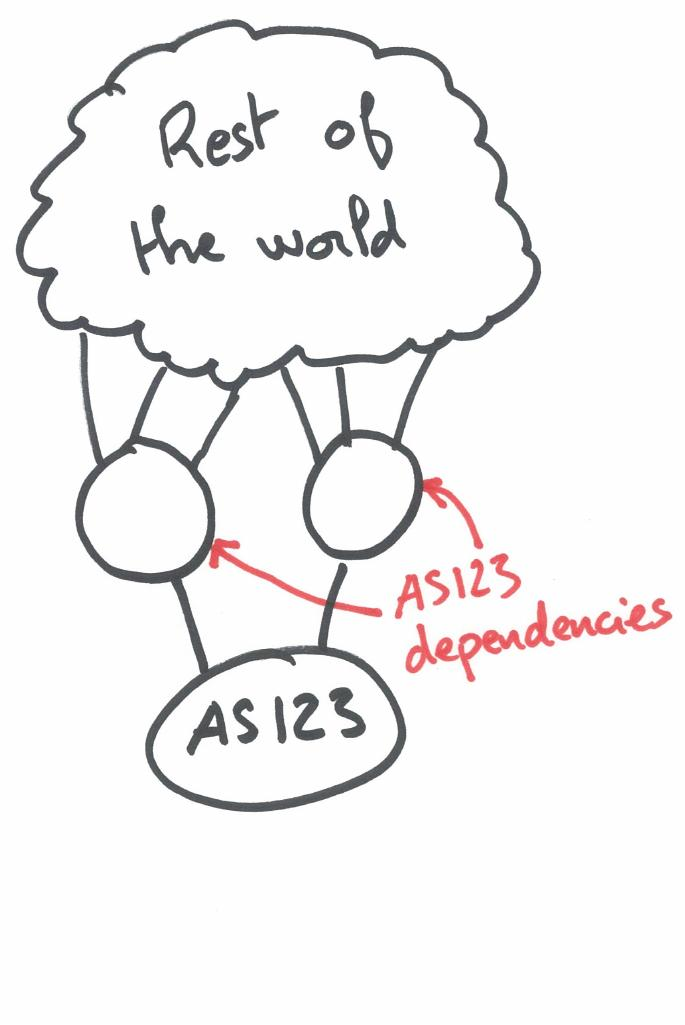
\includegraphics[width=\columnwidth]{./fig/intro.jpg}\\
    \end{columns}
}

\frame{
    \frametitle{Summary}
    \begin{block}{Internet Health Report}
        \begin{itemize}
            \item Monitor connectivity issues
            \item Delay, disconnection and routing anomalies 
            \item \url{https://ihr.iijlab.net}
            \item romain@iij.ad.jp
        \end{itemize}
    \end{block}
    \begin{block}{References}
        \scriptsize{
        \begin{itemize}
            \item A. Shah et al.  "Disco: Fast, good, and cheap outage detection", TMA'17.
            \item R. Fontugne et al. "Pinpointing Delay and Forwarding Anomalies Using Large-Scale Traceroute Measurements", IMC'17.
            \item R. Fontugne et al. "The (thin) Bridges of AS Connectivity: Measuring Dependency using AS Hegemony", PAM'18.
        \end{itemize}
        }
    \end{block}
}

\appendix
\backupbegin

\frame{
    \frametitle{Backup}
}

\frame{
    \frametitle{Online Results: Examples in 2018}
    \begin{block}{Internet Health Report: \url{https://ihr.iijlab.net}}
        \begin{itemize}
            \item DoS attack 
                \begin{itemize}
                    \item \href{https://ihr.iijlab.net/ihr/36459/asn/?date=2018-03-03\&last=7\&hegemonydate=2018-02-28+17\%3A00\&hegemonyy=y}{Attack against Github on Feb. \nth{28}}
                    \item \href{https://ihr.iijlab.net/ihr/52062/asn/?date=2018-03-21\&last=7\&hegemonydate=2018-03-18+07\%3A45\&hegemonyy=y}{Attacks during Russian elections Mar. \nth{18}}
                \end{itemize}
            \item Outage
                \begin{itemize}
                    \item \href{https://t.co/3IinuuJoQN}{Power outage in northern Brazil, Mar. 21st}
                    \item \href{https://t.co/oesCp6OuvK}{DECIX outage, Apr. 4th}
                    \item \href{https://t.co/LrGb46lYjY}{The fall of Bitcanal (\emph{the Hijack factory}), July}
                \end{itemize}
            \item BGP leak
                \begin{itemize}
                    \item \href{https://t.co/VQmo7MHV3p}{Leak from CloudFlare, Jul. 1st}
                \end{itemize}
            \item Censorship
                \begin{itemize}
                    \item Country-level bottlenecks: \href{https://t.co/XDpnL1AeLF}{Iran}, \href{}{China}, \href{}{Pakistan}, ...
                    \item \href{https://ihr.iijlab.net/ihr/28761/asn/?date=2013-09-16&af=4}{CrimeaCom in 2013} vs. \href{https://ihr.iijlab.net/ihr/28761/asn/?date=2018-09-16&af=4}{CrimeaCom in 2018}
                    \item \href{https://t.co/wPyakXfut4}{Exams in Iraq, June}
                    \item \href{https://t.co/2ixTJsHPCa}{Protests in Iraq, Jul. 14-15th}
                \end{itemize}
        \end{itemize}

    \end{block}
}

\frame{
    \frametitle{Google}
        \begin{columns}
            \column{.5\textwidth}
            IPV4 local graph:
            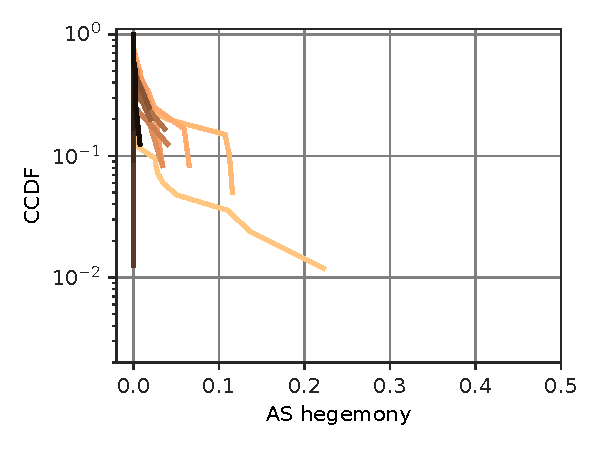
\includegraphics[width=\columnwidth]{./fig/longitudinalAS15169.pdf}
            \column{.5\textwidth}
            IPv6 local graph:
            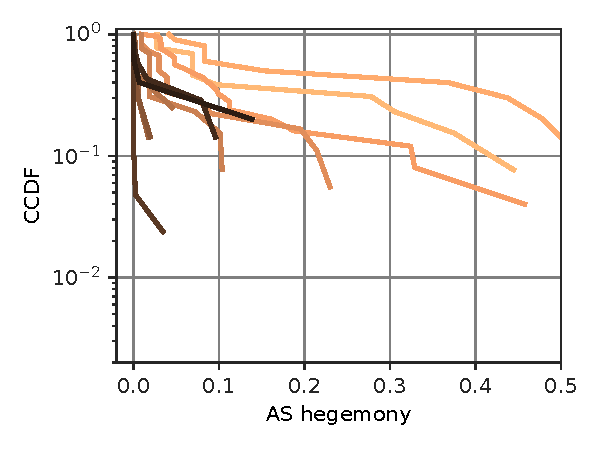
\includegraphics[width=\columnwidth]{./fig/longitudinalAS15169_ipv6.pdf}
        \end{columns}
        \begin{center} 
            
\includegraphics[width=.5\columnwidth]{./fig/longitudinallegend2.pdf}

            \textcolor{red}{ $\rightarrow$  }
        \end{center}
}

\frame{
    \frametitle{Akamai}
        \begin{columns}
            \column{.5\textwidth}
            IPV4 local graph:
            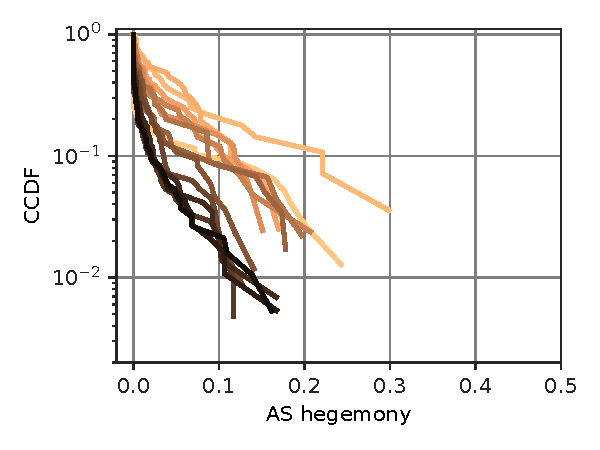
\includegraphics[width=\columnwidth]{./fig/longitudinalAS20940.pdf}
            \column{.5\textwidth}
            IPv6 local graph:
            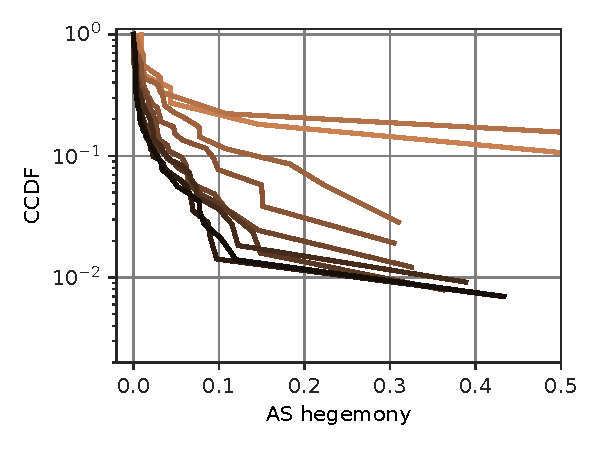
\includegraphics[width=\columnwidth]{./fig/longitudinalAS20940_ipv6.pdf}
        \end{columns}
        \begin{center} 
            
\includegraphics[width=.5\columnwidth]{./fig/longitudinallegend2.pdf}

            \textcolor{red}{ $\rightarrow$  }
        \end{center}
}


\backupend
\end{document}
